\documentclass[aps, secnumarabic, balancelastpage, asmath, amssymb, nofootinbib, floatfix,]{revtex4-2}
\usepackage[titles]{tocloft}
\usepackage[newfloat]{minted}
\usepackage{graphicx}
\usepackage{float}
\usepackage{caption}
\usepackage{siunitx}
\usepackage[export]{adjustbox}
\usepackage{subcaption}
\usepackage{amsmath}
\usepackage{hyperref}
\usepackage{subcaption}
\usepackage{tikz}
\usepackage{multirow}
% \usepackage[table,xcdraw]{xcolor}
\usepackage{xcolor}
\usepackage{cprotect}
\usepackage{verbatimbox}
\usepackage{listings}
\usepackage{xparse}
\usepackage{listings}
\usepackage{paralist}
\usepackage[export]{adjustbox}
\usepackage{svg}
\usepackage{xurl}
%\usepackage{times}
\NewDocumentCommand{\codeword}{v}{%
\texttt{\textcolor{black}{#1}}%
}

\hypersetup{colorlinks=true, pdfstartview=FitV, linkcolor=blue, citecolor=black, plainpages=false, pdfpagelabels=true, urlcolor=black}

\newenvironment{code}{\captionsetup{type=listing}}{}
\SetupFloatingEnvironment{listing}{name=Source Code}

\definecolor{backcolour}{rgb}{0.95,0.95,0.92}
\definecolor{mGreen}{rgb}{0,0.6,0}
\definecolor{mGray}{rgb}{0.5,0.5,0.5}
\definecolor{mPurple}{rgb}{0.58,0,0.82}
\definecolor{backgroundColour}{rgb}{0.95,0.95,0.92}
\definecolor{LightGray}{gray}{0.9}

\setlength{\arrayrulewidth}{0.3mm}
\setlength{\tabcolsep}{5pt}
\renewcommand{\arraystretch}{1.5}
\graphicspath{{./image/}}

\usepackage{setspace}
\usepackage{titletoc}
%\contentsmargin{2.55em}
\dottedcontents{chapter}[1.5em]{}{2.3em}{1pc}
\dottedcontents{section}[1.5em]{}{1.7em}{0.5pc}
\dottedcontents{subsection}[3.9em]{}{2.4em}{0.5pc}
\dottedcontents{subsubsection}[6.6em]{}{2.7em}{0.5pc}
\dottedcontents{paragraph}[10.2em]{}{3.5em}{0.5pc}

\usepackage{etoolbox}
\makeatletter
\pretocmd{\chapter}{addtocontents{toc}{\protect\addvspace{15\p@}}}{}{}
\pretocmd{\section}{\addtocontents{toc}{\protect\addvspace{9\p@}}}{}{}
%\pretocmd{\subsection}{\addtocontents{toc}{\protect\addvspace{15\p@}}}{}{}
\makeatother


\stepcounter{secnumdepth}
\stepcounter{tocdepth}

% Usual (decimal) numbering
\renewcommand{\thesection}{\arabic{section}}
\renewcommand{\thesubsection}{\thesection.\arabic{subsection}}
\renewcommand{\thesubsubsection}{\thesubsection.\arabic{subsubsection}}

% Fix references
\makeatletter
\renewcommand{\p@subsection}{}
\renewcommand{\p@subsubsection}{}
\makeatother

\lstset
{ %Formatting for code in appendix
    basicstyle=\footnotesize,
    numbers=left,
    stepnumber=1,
    showstringspaces=false,
    tabsize=1,
    breaklines=true,
    breakatwhitespace=false,
    %basicstyle=\ttfamily,
    %columns=fullflexible,
    frame=single,
    postbreak=\mbox{\textcolor{red}{$\hookrightarrow$}\space},
    numbersep=5pt,
}

\def\bibsection{\section*{\refname}}
\usepackage{wrapfig}
\usepackage{relsize}
\usepackage{epstopdf}
\usepackage{booktabs}

\def\justifying{%
  \rightskip=0pt
  \spaceskip=0pt
  \xspaceskip=0pt
  \relax
}

\begin{document}
%top matter
    \begin{titlepage}
   \begin{center}
       \vspace*{1cm}

	\Huge
       \textbf{CE323 - Advanced Embedded Systems Design}

       \vspace{0.5cm}

       \LARGE
        \textbf{Assignment Report\\Home Alarm System}

       \vspace{1.5cm}

       \textbf{Akshay Gopinath}\\
       \textbf{Registration Number: 2005614}

   \end{center}
   \tableofcontents
   \listoffigures
\end{titlepage}

%\thispagestyle{plain}
%\Large
%\textbf{Contributions}

%\clearpage

% \thispagestyle{plain}
% \begin{center}
%     \Large
%     \textbf{CE315 - Mobile Robotics}

%     \vspace{0.4cm}
%     \large
%     \textbf{Assignment 1 Report}

%     \vspace{0.4cm}
%     \textbf{Akshay Gopinath}

%     %\vspace{0.9cm}
%     \section*{Abstract}
%     \fontsize{11pt}{12pt}\selectfont

% \end{center}
% \fontsize{11pt}{12pt}\selectfont
% {
% \setlength{\parindent}{0pt}

% {\bf Insert Abstract here}

% }
% \clearpage

% \tableofcontents

%\clearpage

% \listoffigures
% \clearpage

% \listoftables

\clearpage


\section{\fontsize{11.3pt}{12pt}\selectfont \bf Introduction}
\fontsize{11pt}{12pt}\selectfont
\label{sec:1}

{
\setlength{\parindent}{0pt}

This report documents a design of a home alarm system on an Embedded platform. The target embedded device is the ARM mbed LPC1768 development board which houses a 32-bit Cortex-M3 Microcontroller. The software design used is scheduler based, where tasks are configured to run at set refresh rates, allowing for clean, extendable, modular and flexible code.

\subsection{\fontsize{11.4pt}{12pt}\selectfont \bf Requirments Form \label{sec:1.1}}
\setlength{\parindent}{0pt}
{
% \Large
{\bf Name: }Home Alarm System
~\\
~\\
{\bf Purpose: }To prevent uninvited house intrusion by detecting sensor activation within the various zones.
~\\
~\\
{\bf Inputs: }Keypad to enter password, Normally Open/Closed sensors/switches at each zone.
~\\
~\\
{\bf Outputs: }LED to display the system status, LCD screen for user interface.
~\\
~\\
{\bf Function Specifications: }The system has 6 states, unset, exit, set, entry, alarm and report. 
\begin{itemize}
\item \textbf{Unset State: }Activation of sensors should not cause the alarm LED to blink, and entry of the correct passcode will cause a transition to the set state. Entry of wrong passcode will transition to alarm state.
\item \textbf{Exit State: }There is a configurable time interval (exit period) for example 1 minute for evacuation. The alarm LED will be blinking. Entry of correct passcode will transition back to unset state. Transition to alarm state occurs when incorrect code is entered three times or if any sensor is activated. If all sensors are inactive after the exit period expires, the system transitions to the entry state.
\item \textbf{Set State: }Activation of entry/exit zone sensor causes a transition to the entry state. Activation of other sensors will make the system transition to the alarm state.
\item \textbf{Entry State: }The entry period is a configurable time limit, for example 1 minute. The alarm LED will blink. The correct passcode will change the system back to unset state. Activation of any sensor or if the correct password is not entered within the time limit, the system transitions to the alarm state.
\item \textbf{Alarm State: }Alarm LED should be on all the time and switch off after 2 minutes. If incorrect password is entered, the system stays in alarm state, else it transitions to report state.
\item \textbf{Report State: }The LCD screen displays which zones have been triggered (the error code). And the system can be cleared (transition back to unset state) when the enter button is pressed.
\end{itemize}
~\\
{\bf Performance: }The tasks refresh rates in the system have been tuned for optimal performance. The is LCD updated every 200ms, the keypad polling refresh rate is set to 100ms. The sensor/switch task is ran at a rate of 100ms. EDIT TO SHOW IN CODE SNIPPET
~\\
~\\
{\bf Manufacture costs: }Less than £100 including the Microcontroller, LCD screen, keypad and sensors/switches.
~\\
~\\
{\bf Physical size/weight: }The sensors/switches should be sized well to comfortably fit into doors and windows. The user interface (keyboard and LCD) should fit on a house dashboard.
~\\
~\\
{\bf Project Constraints: }Due to the hardware available, switches will represent sensor activation and an LED will represent the alarm. Figure \ref{fig:appendix1} in the appendix shows the hardware used for the project.
~\\
~\\
{\bf Design Parameters: }The software has various configurable paramaters such as exit state and entry state time limit, LCD refresh rate and Keypad poll rate, alarm state LED on time, password, sensor poll rate. EDIT TO SHOW IN CODE SNIPPET


}

\clearpage

\section{\fontsize{11.3pt}{12pt}\selectfont \bf State Machine Diagram}
\fontsize{11pt}{12pt}\selectfont
\label{sec:2}

\begin{figure}[h]
  \centering
  %\captionsetup{justification=centering}
  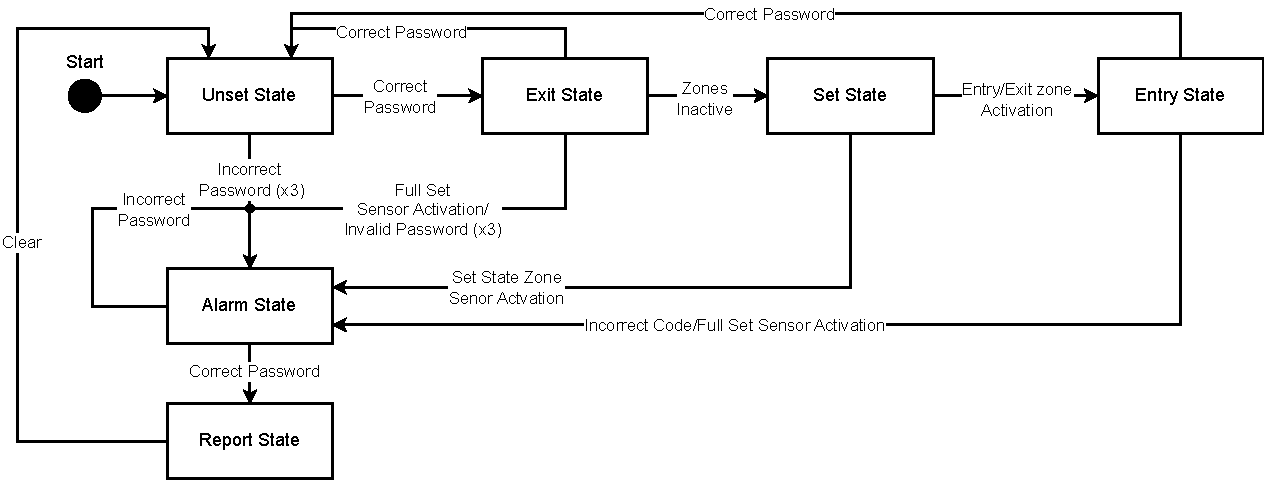
\includegraphics[scale = 0.85]{ce323-state-diagram.pdf}
  \caption{\em State Machine Diagram}
  \label{fig:image1}
\end{figure}

Figure \ref{fig:image1} above represents the state machine diagram of the home alarm system. 



\clearpage

\section{\fontsize{11.3pt}{12pt}\selectfont \bf Class Diagram}
\fontsize{11pt}{12pt}\selectfont
\label{sec:3}


\begin{figure}[h]
  \centering
  %\captionsetup{justification=centering}
  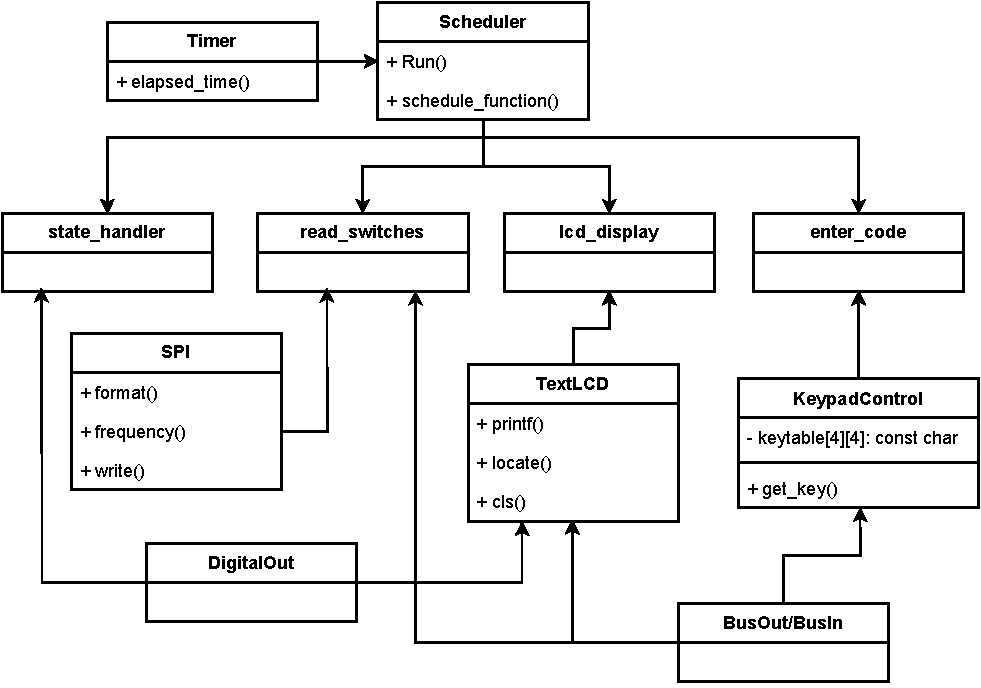
\includegraphics[scale = 1.1]{class.drawio.pdf}
  \caption{\em Class Diagram}
  \label{fig:image1}
\end{figure}



\clearpage

\section{\fontsize{11.3pt}{12pt}\selectfont \bf Sequence Diagram}
\fontsize{11pt}{12pt}\selectfont
\label{sec:4}

\begin{figure}[h]
  \centering
  %\captionsetup{justification=centering}
  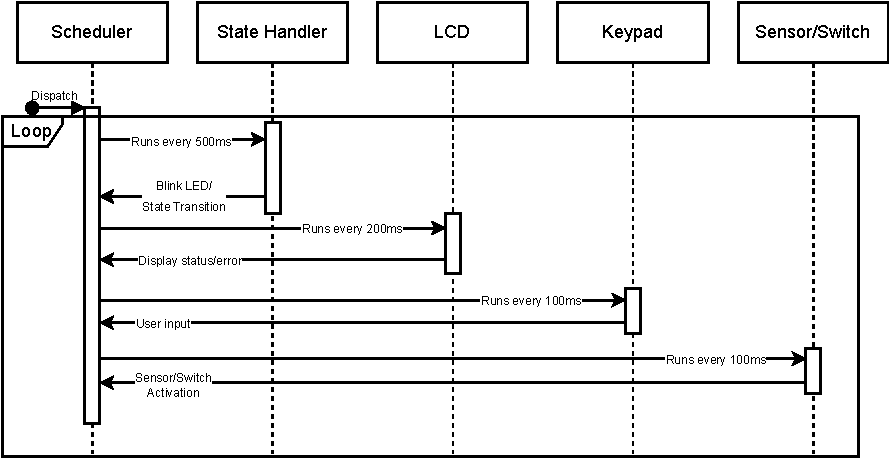
\includegraphics[scale = 1.2]{seq.drawio.pdf}
  \caption{\em Sequence Diagram}
  \label{fig:image1}
\end{figure}



\clearpage

\section{\fontsize{11.3pt}{12pt}\selectfont \bf Appendix}
\fontsize{11pt}{12pt}\selectfont
\label{sec:5}


}
% Appendix

\end{document}